\textbf{Overall narrative should be:}

Dark matter is one of the clearest indications of physics beyond the Standard Model.

The absence of a confirmed WIMP signal motivates complementary searches in lower-mass regions.

LDMX targets light dark matter using a missing-momentum fixed-target strategy.

This requires identifying rare signal-like events in a detector environment where pile-up and backgrounds complicate reconstruction, but it also provides an opportunity if one can analyze these events as well!

Modern ML in HEP is increasingly used for exactly this type of high-dimensional reconstruction and triggering problem.

This thesis explores such an ML-based reconstruction strategy for LDMX.


\subsection{Dark Matter Particle Physics}
\label{sec:dm_particle_physics}


\gls{dm} is an invisible and hypothetical form of matter that does not interact with electromagnetic radiation. \gls{dm} is motivated by astronomical studies and these imply that \gls{dm} has a gravitational interaction with normal matter, i.e the matter that is included in the \gls{sm} of particle physics. Yet there are no experiments on Earth that have been able to detect \textit{\gls{dm} particles}, prove the creation of \gls{dm}, or prove a theory that explains \gls{dm} at the subatomic level. In cosmology \gls{dm} is a widely accepted explanation for observed gravitational effects of celestial bodies that cannot solely be explained by general relativity and normal matter. The bridge of \gls{dm} in cosmology to particle physics has not been trivial. By modern standards, however, this pressing discrepancy between \gls{dm}'s clear presence in cosmology and \gls{dm}'s absence in particle physics is perhaps the largest reason for why it is considered one of the largest unsolved problems in modern physics. \cite{bertone2016-history-dark-matter} \cite{cirelli2026-darkmatter} 

This subsection will give the reader a brief historical context to \gls{dm} and its introduction in particle physics, an introduction to the thermal freeze out framework that gives thermal relic \gls{dm}, and lastly a description of the Dark Bremsstrahlung particle interaction that is the basis for the \gls{ldmx}.

\subsubsection{Brief History of the Dark Matter Problem}
\label{sec:history}



\textbf{https://www.physicsforums.com/insights/knut-lundmark-prehistory-dark-matter/}

\textbf{This was written long ago. It is way too long, it is not brief as the title says but it should become brief. Pick out the most relevant parts for my story and for my thesis (\gls{dm} particle physics history and how the transition from cosmological scale to subatomic scale is not trivial, even though someone by modern standards could think so). Only the basics should be included, but I would also somehow want to include the story of physicists using the latest available tools to expand physics reach, as that is a cool/cliché story to tell with my thesis in particular (where ML is a ''new'' tool).}

\gls{dm} as a concept encapsulates the idea of matter that exists, but cannot be perceived by ordinary means. In that sense, \gls{dm} as a concept has been around for a long time not only in physics, but also in natural philosophy even preceding the scientific framework. \cite{bertone2016-history-dark-matter}

Galileo Galilei (17th century) looked out in space with his telescope and measured that the movement of Jupiter had irregularities, implying the presence of satellites of unseen mass orbiting it. Galileo deduced that Jupiter likely had 4 moons orbiting it, thus explaining the observed phenomenon, even though they were not directly observable with the naked eye. \cite{bertone2016-history-dark-matter}
%Much of Galileo’s work throughout his life questioned the existing framework of natural philosophy and the geocentric model, where the Earth was in the center of the solar system. His work with the telescope would lay the foundation for the heliocentric model, where the Sun is in the center instead, and in time this would replace the geocentric one. 

As physics progressed, and astronomers got new frameworks and better tools to observe the universe, new questions and problems emerged. By the time of the mid 1850’s Newton’s laws of motion and gravity was a well established framework to determine the gravitational mass of celestial bodies. Within this framework physicists like Le Verrier struggled to explain the orbit of Mercury, which led to a hypothesized planet called "Vulcan" that could solve the problem. Vulcan, which one could perhaps call a "dark planet", was invisible because it did not exist; the solution Le Verrier was looking for was not found until Einstein's theory of general relativity of the 20th century in which the orbit of Mercury around the sun could be predicted without anomalies. \cite{bertone2016-history-dark-matter}

These stories acts for us as early analogies to the concept of \gls{dm}. In the frontiers of science, with the newest technology available, new forms of matter may be revealed that were previously invisible, and the existence new invisible matter be implied as well. There is yet not an etymological reference to the word of "\gls{dm}", but the earliest recorded mentions of the word would emerge at the start of the 20th century. \cite{bertone2016-history-dark-matter}

Henri Poincaré wrote in 1906 about “matiére obscure” (\gls{dm}) when discussing Lord Kelvin’s novel idea of modeling the stars of the Milky Way as a gas of particles. Borrowing ideas from thermodynamics and applying it to astronomy, which would later become a foundational framework in astronomy for \gls{dm} studies, gave a relationship between the size of the system and the velocity dispersion of the stars, in which measurements provided an upper limit to the mass of the Milky Way. The upper limit was distinctly higher than the visible amount of stars, and if one would assume the upper limit of mass to be true, then it would imply dark bodies to explain the discrepancy. Poincaré argued that the upper limit and the implied amount of \textit{\gls{dm}} to exceed the amount of shining matter seemed like an unlikely scenario, a conclusion not unlikely to make considering even shining mass can sometimes be dim and faintly visible. \cite{bertone2016-history-dark-matter}

Fritz Zwicky was a Swiss-American astronomer in the 1930's and was a pioneer in the emerging (though not yet widely accepted) field of \gls{dm}. He was the first one to apply the virial theorem from thermodynamics to determine the mass of a galaxy cluster and when he applied it to the velocity dispersion derived from redshift measurements of the Coma galaxy cluster he found an unusually large estimation of mass, since the velocity dispersion was also unusually large. The observed mass of the cluster predicted an average velocity dispersion of 80 km/s, but the observed average velocity dispersion was 1000 km/s. Upon this discovery, Zwicky famously wrote 

\begin{center}
\textit{"If this would be confirmed, we would get the surprising result that \gls{dm} ('dunkle Materie') is present in much greater amount than luminous matter."}
\end{center}

Still today, about 90\% of the mass of the Coma cluster is estimated to consist of \gls{dm}. The Coma galaxy cluster is one of the first most prominent examples of an astronomical gravitational anomaly that implies the presence of invisible \gls{dm}. As for the universe as a whole, it is estimated that \gls{dm} makes up about 84\% of the total mass of the universe. 

In the scope of the latest decades in physics there has undergone a transition of \gls{dm} mainly referring to unseen matter in the universe in the context of astrophysics to also include \gls{dm} in the context of particle physics. The inclusion of \gls{dm}'s relevancy in particle physics has not always been accepted by the scientific community. As Bertando et al. describes it, cosmology was considered merely half a century ago something of a ''fringe-science'', due to a perceived lack of little predictive power or testability. 

Today however, \gls{dm} has been attempted to be explained by finding a \gls{dm} particle that could fit into the framework of the \gls{sm}. This shift of \gls{dm} research stems perhaps mainly from the fact that baryonic \gls{dm} is simply not compatible with observations any longer. Baryonic \gls{dm} is normal matter that are not stars or otherwise luminous. Baryonic \gls{dm} solutions to the \gls{dm} problem akin the ones of Galileo’s days of unseen moons of Jupiter are not possible anymore and and the ''unlikely'' possibility of a \gls{dm} exceeding the amount of shining matter of Poincaré's days have become instead the likely scenarios. The exclusion of baryonic \gls{dm} are based on two main observational truths: 

\begin{itemize}
    \item The amount of baryonic matter in (i.e non-luminous normal matter) needed to make up for the missing mass would cause gravitational lensing in a way that is not observed. 
    \item The cosmic microwave background sets an upper limit on the anmount on the baryonic \gls{dm} in the universe, which is 20\% of total universe mass. 
\end{itemize}

There has has also been other attempts of explanations of the \gls{dm} problems, such as finding a new elegenat model of gravity as with the proposed \gls{mond} (Mordehai Milgrom, 1982) that has been one of the leading candidate solutions that found initial success to explain \gls{dm} phenomenon that does not introduce particle \gls{dm}, but there has also been critical observations difficult to merge with \gls{mond}, thus pointing the way for \gls{dm} candidates in particle physics once again. 

This concludes the historic review for the scope of this paper. The roots of \gls{dm} in modern physics is based in astronomy, and the transition from the cosmological scale in astrophysics to the subatomic scale in particle physics has so far proven to be highly nontrivial.

\subsubsection{Dark Matter Particles}
\label{sec:dm_particles}

Over the last decades the arguments for \gls{dm} particles has become the frontier standard and solutions to the \gls{dm} problem is trying to be found in particle physics. Evidence points to the following key properties must hold true for any \gls{dm} particle candidate:

\begin{enumerate}
    \item \textbf{Mass}
    \begin{itemize}
        \item A \gls{dm} candidate must have mass higher than zero. The mass of \gls{dm} is why it has gravitational influence with other matter, including normal matter included in the \gls{sm}. 
    \end{itemize}
    \item \textbf{Stability}
    \begin{itemize}
        \item There is observational evidence for \gls{dm} in the cosmic microwave background. This implies the existence of \gls{dm} to the early stages of the universe, and thus it must be stable enough to have a long lifetime reaching over the current age of the universe.
    \end{itemize}
    \item \textbf{Almost no interaction with the \gls{sm}}
    \begin{itemize}
        \item The only proven interaction of \gls{dm} with the particles of the \gls{sm} is gravity, which is considered to be the weakest interaction within the \gls{sm}, even so weak it is not even experimentally found or explained by \gls{sm} itself. \gls{dm} has no interaction with the electromagnetic force, and \textbf{\textit{if}} there are any other interactions with the \gls{sm}, then it must be weaker than the interaction strengths already ruled out by experiments. 
    \end{itemize}
\end{enumerate}

\subsubsection{Thermal Relic Dark Matter}
%by a Thermal Freeze-Out Process}
\label{sec:termal_relic}


Thermal relic \gls{dm} posits that the abundance of \gls{dm} in the universe is a relic from the early stage of the universe. The relic \gls{dm} could be explained by a \textit{thermal freeze-out process} and in the thermal freeze-out hypothesis one assumes that the normal matter of the \gls{sm} is an almost entirely separated sector compared to \gls{dm} sector (in line with \textit{3)} from \ref{sec:dm_particles}) where we do not know its particle content. The key part of this hypothesis is that we assume at least some non-gravitational interaction between two sectors exists. Thus, in this hypothesis there exists a ''bridge'' between the two sectors this enables a \textit{coupling} between them, i.e destruction of normal matter to creation of \gls{dm} and vice versa. These are the necessary conditions for the thermal freeze-out process. 

At the early stages of the universe, space was much smaller, and all energy was confined within it, thus implying a high average amount of available energy. These conditions allowed for the creation of mediator particles that coupled the \gls{sm} and the \gls{dm} sectors and these two must thus have been in \textit{thermal equilibrium}. As the universe expanded and cooled down over time, eventually this bridge between the two sectors would close as mediator particles could not be formed and the thermal equilibrium becomes \textit{frozen out}. If \gls{dm} is stable, then the total mass of \gls{dm} from the early stage should be relatively preserved, and this is the \textit{thermal relic \gls{dm}} we observe in the universe today. \cite{du2022-revisiting-freeze-in-freeze-out} 



The thermal freeze out scenario gives a lower and an upper bound on the mass of \gls{dm} particles to XX-XX, which narrows down the search for \gls{dm} particles substantially, please see the energy range in figure \ref{fig:dm_candidate_range}. Within the energy range of thermal \gls{dm} the search for \gls{dm} particles can be even further narrowed down if we restrict the search to the energy range of \gls{ldm}, and this is the energy range of interaction strength that the \gls{ldmx} has narrowed down its search for \gls{dm} candidates by excluding the possibility of the \gls{wimp}. 

\begin{figure}
    \centering
    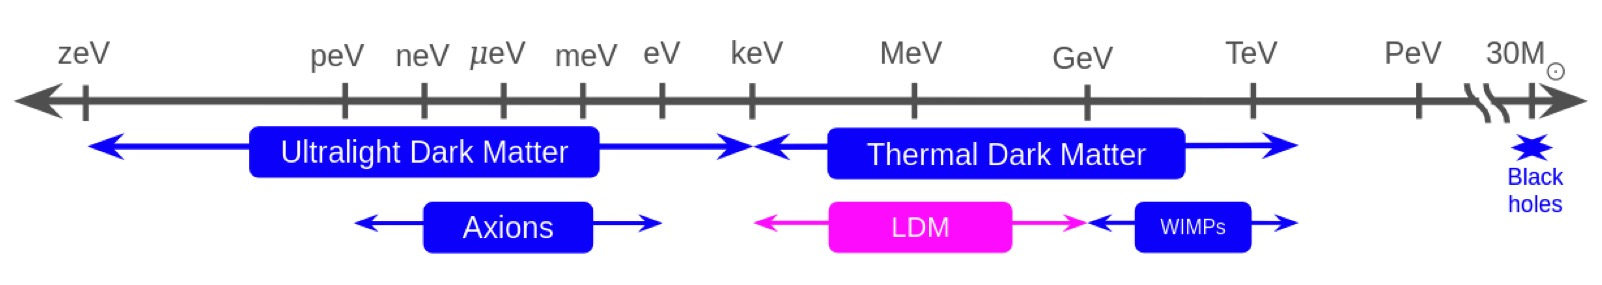
\includegraphics[width=1\linewidth]{config/fig/dm_range.jpeg}
    \caption{Energy ranges of possible DM candidates. Thermal \gls{dm} is in the energy range of XX-XX and the light \gls{dm} energy range is a subset of YY-YY.}
    \label{fig:dm_candidate_range}
\end{figure}




\subsubsection{Dark Bremsstrahlung - A Benchmark Model for LDMX}
\label{sec:dark_brem}

\begin{figure}
    \centering
    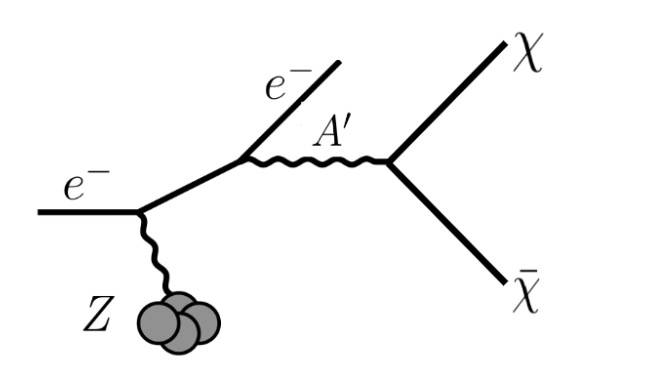
\includegraphics[width=1\linewidth]{config/fig/dark_brem.jpeg}
    \caption{Enter Caption}
    \label{fig:placeholder}
\end{figure}



\subsection{The Light Dark Matter eXperiment}
\label{sec:ldmx}

\gls{ldmx} is an electron fixed-target experiment in particle physics with the intention to probe for \gls{dm} candidates in the sub-GeV mass range, a sector that is still largely unexplored. 
\gls{ldmx} is designed to search for matter production of the dark bremsstrahlung particle interaction through a
\textit{missing momentum} signature, i.e the experiment will search for a loss of energy that matches an expected \gls{dm} interaction strength for a certain \gls{dm} theoretic model. \gls{ldmx} will operate at the \gls{slac} in San Francisco, California using an 8 GeV electron beam and the design of the experiment is motivated by the performance requirements of a high-rate missing momentum search. The unique angle of \gls{ldmx} for \gls{dm} search is enabling sensitivity to MeV-GeV \gls{dm} interaction strengths, thus expanding \gls{dm} search to new energy regions. \cite{akesson2018-ldmx}

As of the time of writing this report, the international collaboration of design and preparation of the experiment is ongoing and it includes development of different areas of the experiment such as: the detectors and sub-detector electronics but also the implementation of algorithms and other computational methods that determines what measurements that will be stored and that analyzes the data measurements \textit{reconstructing} what physical observables took place in the particle event. This section will cover the different parts of the \gls{ldmx} apparatus and corresponding tools for data storage that are relevant to the scope of this report: the tracker subdetector and the electromagnetic calorimiter subdetector and the trigger. 

\subsubsection{LDMX Search for Dark Matter}

\begin{figure}[H]
    \centering
    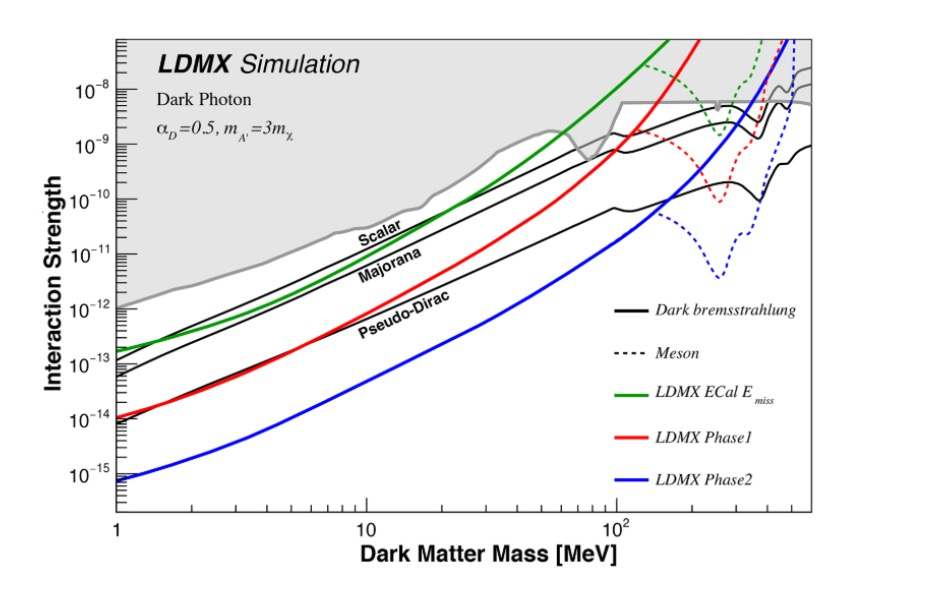
\includegraphics[width=1\linewidth]{config/fig/exclusion_ldmx.jpeg}
    \caption{\textbf{from Aert} Projected exclusion prospects for the different runs of LDMX. Benchmark thermal
relic targets for DM with different particle properties are shown as black lines, and constraints
from previous experiments are represented by the gray area}
    \label{fig:exclusion_ldmx}
\end{figure}

\subsubsection{Detector Setup}

This subsection should give the reader an overview of the entire LDMX detector where the different subdetectors are clearly laid out. The tracker, 


* Include a figure with schematics of the ldmx detector. 

\begin{figure}[H]
    \centering
    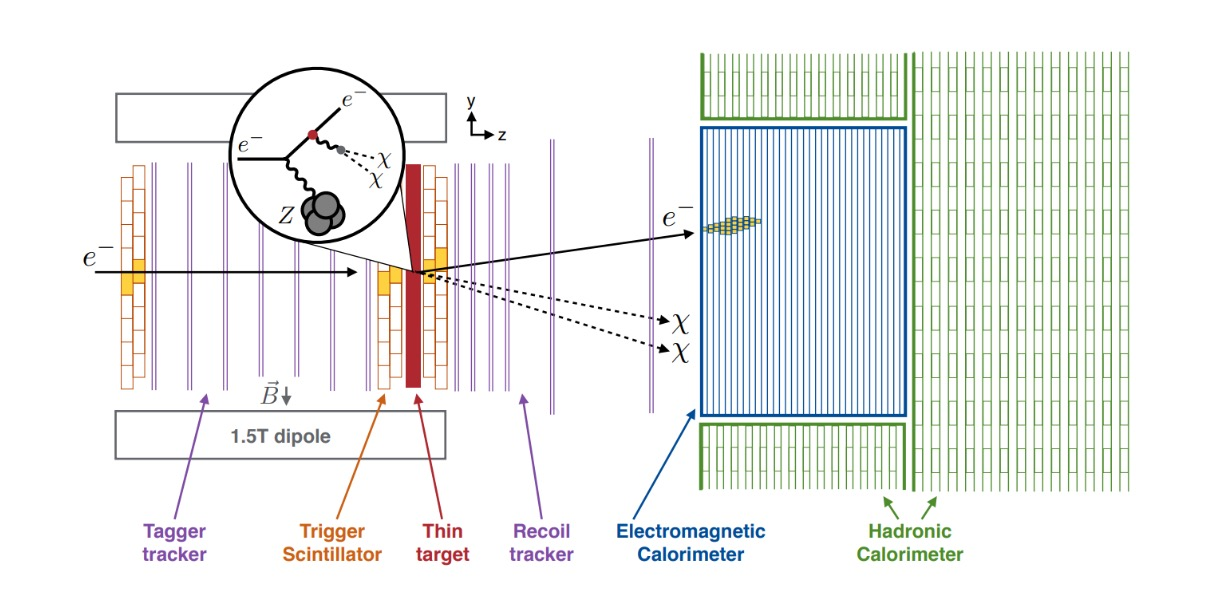
\includegraphics[width=1\linewidth]{config/fig/ldmx_schem.jpeg}
    \caption{A schematic layout of the LDMX detector.}
    \label{fig:ldmx_schem}
\end{figure}

* 

\subsubsection{Electromagnetic Calorimiter}

\begin{figure}[H]
    \centering
    \includegraphics[width=1\linewidth]{config/fig/ecal_cells_and_triggercells.jpg}
    \caption{}
    \label{fig:ecal_cells_and_triggercells}
\end{figure}

This subsection should cover the ECal subdetector. 

* Include a figure with the ECal cells and the trigger cells of the ECal. 

\subsubsection{Tracker and Trigger Scintillators}

This subsection should cover the tracker subdetector including: trigger scintillators, tracker, recoil tracker. 

* Include a figure with the trigger scintillator schematics. The current one and maybe mention the newly proposed one as well. 

\subsubsection{Trigger}

Define the trigger and explain + motivate its purpose. 

-> Also introduce the concept of online and introduce offline analysis

\subsubsection{Formalism: electrons and detector response as stochastic variables}
\label{sec:formalism}


This section aims to introduce some basic formalism to express the problem that will be studied in mathematical terms, in order to enhance the formulation, but also to enhance the eventual discussion. 

Let \(T^{(k)}\) denote the physical trajectory and shower development of electron \(k\). The propagation of the electrons are, for all intents and purposes, partly stochastic, and partly deterministic. 
The corresponding true energy depositions in the \gls{ecal} are represented by
\[
Z^{(k)} = \{(r^{(k)}_i, E^{(k)}_i)\}_{i=1}^{N_k},
\]
where \(r^{(k)}_i \in \mathbb{R}^3\) is the spatial position of deposition \(i\), 
\(E^{(k)}_i\) is the deposited energy, and \(N_k\) is the number of depositions associated with electron \(k\).

For distinct primary electrons \(k \neq \ell\), the simulated shower developments are treated as independent stochastic processes,
\[
T^{(k)} \perp\!\!\!\perp T^{(\ell)}
\]
Consequently, the corresponding true energy deposition patterns are also treated as independent,
\[
Z^{(k)} \perp\!\!\!\perp Z^{(\ell)}
\]

The detector response is represented by also a stochastic mapping from true energy depositions to observed or reconstructed detector hits. 
Let
\[
\mathcal{H} = \mathcal{R}\!\left(Z^{(1)},\ldots,Z^{(m)}\right)
\]
denote the set of reconstructed \gls{ecal} hits produced after overlay and detector response, where \(\mathcal{R}\) includes effects such as finite detector granularity, energy sharing, thresholds, noise, and reconstruction procedures.

Although the underlying deposition patterns \(Z^{(1)},\ldots,Z^{(m)}\) are treated as independent before overlay, the observed hit collection \(\mathcal{H}\) is not naturally decomposed into independent components. After detector response and reconstruction, energy depositions from different electrons may overlap spatially, contribute to the same reconstructed hit, or become difficult to assign uniquely to their originating electron. 

The ultimate goal of this thesis boils down to predicting the original quantities given the observed hit collection \textit{as efficiently as possible}. Since the problem, given the introduced mathematical model, has inherent ambiguity, perfect accuracy would never be possible.



\subsubsection{Pile-Up and Physics Reach of LDMX}

Explain what reconstruction is

Explain what pile-up is and \textit{WHY} pile-up is both a problem and an opportunity!



\subsection{Machine Learning Methods for Reconstruction in High Energy Physics}
\label{sec:ml_event_reconstruction_hep}


Short introductory text here stating that ML is a topic of rising interest in HEP and refer to output of ML-related papers in HEP. \cite{iml-wg-hepml-livingreview}'. \textbf{I have realized that the relevancy of this section may be heavily questioned... Feel free to input opinions and cherry-pick if there are relevant parts.}


\textbf{text here}

\gls{ml} has become a tool of rising interest in \gls{hep}, driven by the growing complexity of detector data, the need for efficient event selection, and the search for rare signatures of physics beyond the \gls{sm}. At the same time, advances in deep-learning methods and accelerator-based computing architectures such as \glspl{gpu} have made increasingly powerful \gls{ml} and non-\gls{ml} approaches practical for scientific workflows \cite{sur2026-heterogeneous-computing}. Machine learning and deep-learning methods are not new in \gls{hep}, but the recent rapid growth of machine-learning applications in particle physics is 
\begin{wrapfigure}{r}{0.50\textwidth}
    \centering
    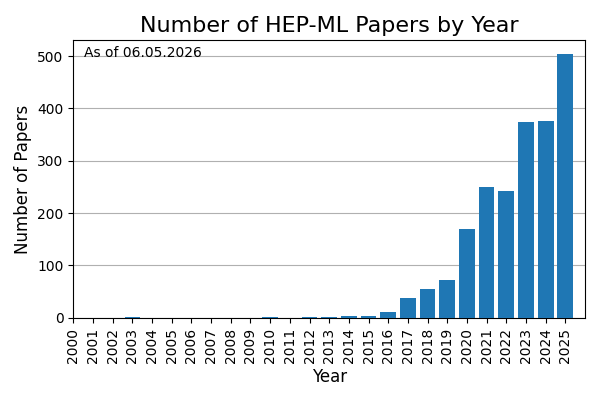
\includegraphics[width=0.48\textwidth]{config/fig/per_year.png}
    \caption{\textbf{Increase the size of labels here} Number of machine-learning-related publications on arXiv in the HEP category per year, based on the Living Review of Machine Learning for Particle Physics \cite{iml-wg-hepml-livingreview}.}
    \label{fig:ml-publications-per-year}
\end{wrapfigure}
reflected both in dedicated reviews and in the continuously updated Living Review of Machine Learning for Particle Physics  \cite{karagiorgi2021-mlnewphysics,feickert2021-livingreview,iml-wg-hepml-livingreview}. Figure \ref{fig:ml-publications-per-year} shows the trend of machine-learning-related publications within \gls{hep} significantly increasing in the last few years. 


The underlying motivation for \gls{ml} in \gls{hep} is that such tools may increase the \textit{physics reach} of experiments, meaning their ability to probe weaker signals, rarer processes, or more challenging regions of parameter space, either by improving sensitivity enabling new discoveries or by making reconstruction and selection more computationally efficient. 

\paragraph{Reconstruction} Reconstruction in \gls{hep} refers to reconstructing the physical interpretables from a measured particle event based on the detector outputs.  Modern \gls{hep} experiments produce high-dimensional and heterogeneous data, where each event may contain a variable number of detector signals distributed across several subdetectors. This makes reconstruction a quite natural application area for machine learning: the task is to transform heterogeneous low-level or intermediate detector information, such as hits, tracks, and calorimeter clusters, into physically meaningful quantities that can be used for triggering, event selection, and analysis.



A useful way to view reconstruction is as an approximate inverse problem. In simulation, a detector may be regarded as a map from an underlying particle-level event to a set of detector measurements. If the particle-level event, representing the physical ''truth'', is denoted by \(Y\), and the corresponding detector response by \(X\), the simulation can be written schematically as
\begin{equation}
    S(Y) = X ,
\end{equation}
where \(S\) represents the detector response. Reconstruction, denoted $R$,  then attempts to inverse the mapping, i.e
\begin{equation}
    R(X) \approx S^{-1}(X) = Y .
\end{equation}
In practice, this inverse is imperfect and often ambiguous, based on the fact that some information is always lost, has stochastic evolutions or only indirectly observed: detector signals have finite resolution and particles may overlap in the detector. These cases does not exclude relevance however, as it could also be useful to study these scenarios as well and infer where our tools of measurement might simply not be enough. Machine-learning-based reconstruction approaches formulate parts of this inverse problem as a learnable mapping from detector-level inputs to physics-level targets, typically using simulated events where truth information is available to us and constructing target information is completely feasible.

\subsubsection{Computational Context in Experimental High Energy Physics}

\textbf{Let Nairit read this section!}

The computational setting of \gls{hep} is also important for understanding the interest in machine-learning-based reconstruction. Large-scale \gls{hep} computing has traditionally been dominated by distributed, \gls{cpu}-based workflows. \cite{sur2026-heterogeneous-computing} This is natural because collision or fixed-target events often are, to a good approximation, independent processes, analog to the electron case of \gls{ldmx} $Z^{(k)} \perp\!\!\!\perp Z^{(\ell)}$ where $k \neq l$, following the notation introduced in Section~\ref{sec:formalism}. Simulation, reconstruction, and analysis can therefore often be parallelized over events with relatively little communication between tasks, making \gls{cpu} clusters and grid computing highly effective, somewhat bypassing an immediate need of software engineering concurrency, which explains the longevity and success of this computing paradigm within \gls{hep}.

At the same time, the wider computing landscape has shifted toward heterogeneous architectures, in particular \glspl{gpu} and other accelerator \footnote{``Accelerator'' in this context refers to specialized hardware such as \glspl{gpu} or even \gls{ml} specialized architectures such as the relatively new \gls{tpu} designed by Google that accelerate the speed of computation for applicable processes\cite{needed}}
-based systems. This development is strongly connected to modern machine learning, where many operations reduce to dense linear algebra and can be executed efficiently on massively parallel hardware, including both training and inference tasks of deep learning \gls{ml} models.

This shift creates both a challenge and an opportunity for \gls{hep}. Rule-based reconstruction algorithms have often been designed around detector-specific logic and sequential or iterative procedures. Such algorithms can be highly effective, but they may be difficult to port efficiently to accelerator hardware and may scale poorly with detector occupancy. Machine-learning models, by contrast, often express reconstruction as a fixed sequence of tensor operations, making inference naturally suited to \glspl{gpu} or other accelerator architectures. 

\subsubsection{MLPF, a Recent Example of ML-based Reconstruction in HEP}

All of the above stated reasons creates a modern context that make up the underlying motivations behind the \gls{mlpf} reconstruction method, designed for the \gls{cms} experiment and the incoming \textit{high luminosity phase} of the \gls{lhc}. The original \gls{mlpf} study published in 2021 used a graph-neural-network-based architecture for efficient particle-flow reconstruction in high-pile-up conditions \cite{pata2021-mlpf}. The latest implementation from early 2026 demonstrates a transformer-based \gls{mlpf} algorithm integrated into the \gls{cms} reconstruction software and evaluated on both simulation and collision data \cite{pata2026-mlpf}. In the latter study, modern hardware, transformer-based computational architectures and recent progress of  the transformer architecture are explicitly part of the motivation for scalable reconstruction in high-dimensional, variable-size event data.

The \gls{mlpf} showcases the motivation for \gls{ml} based reconstruction quite perfectly combining all of the above stated reasons for why \gls{ml} methods have sparked an interest. The \gls{mlpf} uses the modern model architecture, compute is accelerated with modern hardware, the method shows promise of improved speed of compute, resolution of reconstruction and it is motivated by the context of \gls{lhc} high luminosity phase, which will increase complexity with a much higher rate of pile-up.

For the purpose of this thesis, the most relevant role of machine learning is therefore not only as a final classifier that separates signal-like and background-like events, but as a possible reconstruction method. Traditional reconstruction algorithms are often built from physics-motivated rules and detector-specific heuristics. Such methods remain essential, but they may become difficult to optimize in environments with high occupancy, irregular detector geometry, or overlapping detector signatures. Machine-learning-based reconstruction instead attempts to learn parts of the reconstruction mapping $R(X) \approx S^{-1}(X) = Y$ directly from simulated or measured data. It is also important to understand that rule-based and \gls{ml} reconstruction is not either/or, they are the most effective when they work in junction and complement each other. The \gls{mlpf} model takes some object-level inputs that are the results of rule-based reconstruction intermediate outputs such as clusters and particle candidates, in which the \gls{ml}-based \gls{mlpf} can utilize for stronger inference results \cite{pata2021-mlpf}. 

\subsubsection{The GNN and the Transformer under Pile-Up Conditions}

\gls{ml}-based methods are perhaps the most relevant under pile-up conditions, where detector hits from several particles or interactions may overlap and where the association between detector activity and the underlying particle origin becomes ambiguous. In this setting, a model that operates directly on hit-level or object-level detector information may provide additional information beyond a purely rule-based reconstruction, for example by assigning hit-level probabilities or by learning correlations that may be difficult to capture manually with code. One must still remember however that \gls{ml}-methods are certainly also based on ''rules'' in the end, the strength of these methods in this context lie in that their discovery of efficient, or even \textit{optimal} ''rules'', are somewhat automatic and a researcher can explore the space of solutions efficiently.

Architectures such as \glspl{gnn} and \textit{transformer} are particularly well suited to this type of problem because they can operate on variable-size collections of detector objects and learn correlations between them without requiring the data to be arranged on a regular grid. This is important for particle detectors, where the relevant information is often distributed over irregular detector geometries and across multiple subdetectors. By contrast, architectures such as \glspl{cnn} are naturally adapted to regularly spaced image-like data and therefore impose an inductive bias that is not always well matched to detector readout. Graph-based models instead allow calorimeter hits, clusters, tracks, or other detector objects to be represented as nodes, with edges describing geometrical proximity or learned relationships. Transformers provide a related approach but it uses different analogies than nodes and edges. 

In this thesis, the same general motivation is applied to the \gls{ldmx} setting. The aim is not to perform full general-purpose particle-flow reconstruction, as in \gls{cms}, but to build and study a reconstruction platform for identifying electron-induced activity in the electromagnetic calorimeter down to hit-level statistics, especially under pile-up conditions. This is the regime where reconstruction ambiguities are expected to be most relevant, and where machine-learning methods may offer the largest benefit over rule-based approaches.

\textbf{This is kind of outdated, should I include all of this or not?} The rest of this subsection introduces the machine-learning context needed for the reconstruction study in this thesis. First, the existing rule-based reconstruction chain in \gls{ldmx} is reviewed, with emphasis on clustering, particle-flow-inspired reconstruction, and the distinction between online and offline reconstruction. The existing machine-learning-based veto strategy in \gls{ldmx} is then briefly discussed, since it represents an already planned use of machine learning in the experiment \textbf{not relevant for my study?}. The subsection then turns to machine-learning-based reconstruction in \gls{cms}, in particular the development of \gls{mlpf}, which provides a useful point of comparison for the approach studied here. Finally, the basic ideas behind \glspl{gnn} and transformers are introduced and compared. These architectures form the methodological basis for representing calorimeter hits and other detector objects as unordered sets of nodes or tokens, allowing event reconstruction to be formulated as a learnable mapping from detector-level inputs to physics-level targets.

\textbf{Further motivation of why not to use CNN to use somewhere maybe:}

This representation preserves individual detector objects rather than
projecting the event to an image. The number of hits is event dependent, the
\gls{ecal} is three-dimensional, and overlapping showers need not be aligned
with a fixed rasterization. Moreover, trigger-pad-track information is not an
\gls{ecal} pixel quantity. Sets, learned graphs and attention-based token
sequences provide natural ways of relating these heterogeneous objects while
remaining insensitive to an arbitrary ordering of the input rows.


\subsubsection{Rule-Based Reconstruction in LDMX}

Introduce clustering and reconstruction pipelines. Describe existing LDMX reconstruction approaches (CLUE, PF).

Discuss online vs offline reconstruction context in order to give the reader an idea of online/offline and where this reconstruction method aims to relate.

\subsubsection{ML-based Veto in LDMX}

Briefly explain and overview the particle-net implementation that is in place for LDMX. 

%\subsubsection{CLUE}

%\subsubsection{ParticleFlow}

\subsubsection{ML-based Reconstruction in CMS}

Cover MLPF and ParticleNet here. \textbf{Or Skip? }

*Figure flowchart of where the different alternatives of reconstruction (Rule based CLUE, PF and ML) fit in the reconstruction pipeline of LDMX* \textbf{Outdated? Likely skip this}


%Beyond physics performance, the \gls{mlpf} studies are relevant because they connect reconstruction algorithms to modern heterogeneous computing. The original graph-based \gls{mlpf} work emphasized scalable graph construction and accelerator-friendly inference \cite{pata2021-mlpf}, while the later \gls{cms} implementation demonstrated that a transformer-based reconstruction model can be integrated into the \gls{cms} software framework and evaluated on \gls{gpu} hardware \cite{pata2026-mlpf}. This makes \gls{mlpf} an example not only of machine-learning-based reconstruction, but also of how reconstruction algorithms may adapt to the changing computational architecture of \gls{hep}.

\subsubsection{The Graph Neural Network}

Explain the prospect of GNN and discuss advantages compared to CNNs/RNNs for irregular geometries.

Explain why calorimeter data can naturally be represented as graphs. Explain how data from other subdetectors can be included in the same graph representation and refer to MLPF by CMS.

Introduce graph representations and message passing.

Explain \textsc{GravNet}

Explain \textsc{GraphNetConvolution} \cite{qasim2019-gravnet}

Discuss hit-level vs cluster-level inputs.

Explain graph construction: edge definitions, distance metrics, kNN or radius graphs or perhaps fully connected.

*Figure illustrating input possibilities could be nice here*

\subsubsection{The Transformer}

First give the necessary background to the \textsc{Transformer} and the basics of it and how it is structured.

Explain Query, Key, Value. Explain the input (tokens). Explain what the transformer learns. 

Very briefly mention the transformer's extreme rise in popularity seen with the rise of LLMs, how it has expanded from pure natural language processing (NLP) applications to and \textbf{(the last thing here is mentioned in the analogy chapter)} the prediction in the direction of compute architectures.


\subsubsection{An analogy between the Transformer and the GNN}

The Transformer is actually a special case of a \gls{gnn}, and this analogy is relevant to be aware of. The name \gls{gnn} refers to a large catalogue of different implementations but what they all have in common that the input has a suitable analogy as being seen as nodes in a graph in the learned representation of the network, and then message parsing is performed along these. The input to a transformer are called tokens, or even sloppily called words in the context of natural language processing, but one can mathematically show how a generic \gls{gnn} could be molded into an equivalent network of a transformer, something Chaitanya K. Joshi has derived \cite{joshi2025transformersgnn}, but perhaps making the distinction around the terms nodes and tokens more diffuse. 

There is also another \gls{gnn} architecture that is kind of the middle ground of a generic \gls{gnn} and the transformer, known as \gls{gat}, which implements the attention mechanism to \gls{gnn}s, but the attention is not applied globally and being still restricted to local neighborhoods. The derivation in Joshi's paper molds a \gls{gnn} into a transformer by considering a \gls{gnn} with a fully connected graph (i.e, global) and also implementing the attention mechanism to it, obtaining a mathematical equivalent between the two networks \cite{joshi2025transformersgnn}. 

The architectural differences between the two networks might have been blurred, but the transformer architecture has one benefit over the \gls{gnn} currently, namely of \textit{''winning the hardware lottery''} \footnote{The term, introduced by Sara Hooker, describe when a
research idea in computer science wins because it was suited to the available software and hardware and not because the idea is superior to alternative research directions. \cite{hooker2020hardwarelottery}}. There is one practical difference between the two classes, and that is that 
the self-attention mechanism for all tokens in
an input set $\mathscr{S}$ can be computed in a highly parallelized manner as follows:

\[
\widetilde{\mathbf{H}}^{\ell}
=
\operatorname{softmax}
\left(
\mathbf{H}^{\ell}{W}_{Q}^{\ell}
\left(
\mathbf{H}^{\ell}{W}_{K}^{\ell}
\right)^{\top}
\right)
\left(
\mathbf{H}^{\ell}{W}_{V}^{\ell}
\right).
\]

Where $\mathbf{H} \in \mathbb{R}^{n \times d}$ is a matrix of initial representations. 
\textbf{(i took these snippets directly and I dont know how much I want to include or how I can condense)} 
\textbf{snippet 1:} Transformers implement global multi-head attention through highly optimized dense matrix multiplication operations that leverage the parallel processing capabilities of modern \gls{gpu}s and \gls{tpu}s. \cite{joshi2025transformersgnn}.
\textbf{snippet 2:} The multi-head attention mechanism can also be similarly parallelized by performing a single linear
transformation for all heads in parallel, followed by reshaping the queries, keys, and values per head
to tensors of dimension n×k×d/k each. The token-wise operations which follow multi-head
attention are independent of other tokens and trivially parallelizable as well.
In contrast, GNNs typically perform sparse message passing over locally connected structures, which
is substantially less efficient on current GPUs for typical problem scales (with the exception of very
sparse or billion-scale graphs). This involves maintaining an index of neighbours for each node,
and performing gather and scatter operations to propogate messages [Fey and Lenssen, 2019]. As a
result, GNNs are orders of magnitude slower to train and challenging to scale compared to standard
Transformers on current hardware.

\textbf{My text again:} This means that if one would design one \gls{gnn}-based model and one transformer-based model whose performance on their tasks are equally accurate, then the transformer-based model is, if no other apparent downsides, likely the better choice since inference and training will run faster and more efficient on the modern hardware, at least given the clear current shift in the hardware industry. The speed of inference is also especially important if one would design a \gls{ml}-based online reconstruction model meant for being used, at some capacity, in real-time of the experiment, maybe even in triggering. The aspect of speed on modern hardware is specifically one of the mentioned reasons for why the latest iteration of the \gls{mlpf} model abandoned \gls{gnn}s for transformers instead \cite{pata2026-mlpf}. 



%\textbf{Self critical question and reminder:} How does this subsubsection relate to my thesis?

%\textbf{answers:} Becuase it is a valuable lesson for the reader navigating in this landscape trying to represent detector data as nodes/tokens to know that they are almost exactly the same thing if we look at the transformer! It explains why transformers are interesting as well, since GNNs have had a previously established relevancy in ML HEP, thus transformers are an alternative that should perform quite well. In this analogy context, we should also consider the practical benefits of using a transformer architecture. Hardware is currently being designed for the transformer architecture specifically, thus there are computational benefits of sticking with the transformer architecture instead of relying on message parsing computations of the gnn. This leads to the practical "lemma" that if I would find in my analysis that the models perform equally well in accuracy, then I would recommend the transformer model, which is a very practical and sensible conclusion that I can refer back to! This explains why tokens/nodes are essentially the same. It explains the hardware lottery term it can be resused in discussion. 

%\textbf{Starting Ideas:} The transformer and the gnn architectures are distinct architectures but they also have similarities and one can mold the gnn to essentially become a transformer: there exist an analogy between them and I believe it is revolved around a fully connected graph gnn is essentially a transformer (but without the self attention mechanism?) and vice versa. Explain how a fully connected graph can be compared to a transformer. Explain a transformer and explain the attention mechanism. What is the stepping stone distance going from a GNN to a transformer? Why could that be reasonable? Does it anticipate to introduce new challenges?

%\textbf{comments: explain the attention mechanism should possibly be made earlier? then the reader already understand the math used above}

%*Figure somewhere illustrating the idea of GNN in HEP reconstruction and subdetector data (probably omit if there is a proper one later anyways)*


